\chapter{Implementation and Evaluation}
\label{Implementation_and_Evaluation}
In this chapter, we evaluate the method presented in Chapter 3. First, the environment and the reasons of using them will be explained. Then we will show various experiments and their results.

\section{General setup}
Table~\ref{table:Experiment_table} is a summary of all the tools and their versions. We use Mininet to simulate the data center network \cite{Mininet}. It allows us to create a large-scale virtual network easily. It provides Python APIs as well as a command line interface to customize the network. It also offers an interactive interface to test the connectivity and performance.

\begin{table}[H]
\centering
\caption{Summary of experimental environment}
\begin{tabular}{|l|p{4cm}|p{4.5cm}}
\hline Item & Detail version \\
\hline
\hline Operating system & Ubuntu 14.04 x86\_64 \\
\hline Controller & Ryu\_manager 4.0 \\
\hline Network Emulator & Mininet 2.2.1 \\
\hline Topology generator & Fast Network Simulation Setup (FNSS) 0.6.1\\
\hline Packet Generator & Ryu packet library API \\
\hline Southbound API & OpenFlow 1.3 \\
\hline Virtual switch & OpenvSwitch 2.5.0 \\
\hline 
\end{tabular}
\label{table:Experiment_table}
\end{table}

We evaluate the effectiveness of the detection method in various network topologies, which are generated by Fast Network Simulation Setup (FNSS), a Python module that is able to generate various types of network topology. It not only supports DCN topologies, but also provides the Mininet API, making it easy to import the generated topology into Mininet. The network topologies we use are two-tier topology, three-tier topology and fat-tree topology of various sizes. The number of switches and average degrees (i.e., the number of links between two switches) for each type are shown in Table~\ref{table:network_env}. The numbers in the topology name are parameters such as number of core switches, aggregation switches and edge switches, which characterize the network size. The parameters have the same meaning as the ones in \cite{FNSS}. For example, a fat-tree topology ``fat\_tree\_n'' has $n$ pods, a two-tier topology ``two\_tier\_a\_b'' has $a$ core switches and $b$ edge switches in total, and a three-tier topology ``three\_tier\_x\_y\_z'' contains $x$ core switches and $y$ aggregation switches in total, and each aggregation switch is connected to $z$ edge switches. 

\begin{table}[H]
\centering
\caption{Details of network topologies}
\begin{tabular}{|l|l|l|l|}
\hline topology types & number of switches & average degrees \\
\hline
\hline fat\_tree\_2 & 5 & 2 \\
\hline fat\_tree\_4 & 20 & 4 \\
\hline fat\_tree\_6 & 45 & 6 \\
\hline fat\_tree\_8 & 80 & 8 \\
\hline fat\_tree\_10 & 125 & 10 \\
\hline fat\_tree\_12 & 180 & 12 \\
\hline fat\_tree\_14 & 245 & 14 \\
\hline two\_tier\_6\_14 & 20 & 9.1 \\
\hline two\_tier\_10\_10 & 20 & 10.5 \\
\hline two\_tier\_14\_6 & 20 & 8.7 \\
\hline three\_tier\_2\_3\_5 & 20 & 2.85 \\
\hline three\_tier\_4\_2\_7 & 20 & 2.90 \\
\hline three\_tier\_4\_4\_3 & 20 & 3.40 \\
\hline three\_tier\_5\_5\_2 & 20 & 4.00 \\
\hline 
\end{tabular}
\label{table:network_env}
\end{table}

The in-band control is used for control channel by default in Mininet. Although there are special flow entries for in-band control channel, they are hidden and will not have any influence on our experiment. Only one controller is used. The hosts do not have any functinality to the detection method, only a minimal number of them are assumed in the experiment to make the topology reasonable. In a fat-tree topology, the number of hosts is the number of pods divided by 2, while in two-tier and three-tier topologies, one host is connected to each edge switch. There are 254 flow tables in an OpenFlow switch simulated by Mininet. The flow entries are installed pro-actively in the OpenFlow switches, and the controller will maintain a record of switches, including ports, links and flow entries. The detection packets from the controller should be sent to a normal port rather than the default controller-specifying port \texttt{OFPP\_CONTROLLER}.

The core algorithm of the flow entry detection method is implemented on a Ryu controller. It obtains essential information from the configuration files, finds aggregated groups, generates raw packets, sends them by \texttt{Packet\_out}, and checks \texttt{Packet\_in} to see if the packets come back as expected. Packets are generated by Ryu's built-in API library. To send \texttt{Packet\_out} with a raw packet, the action should be set to ``forwarding to \texttt{OFPP\_TABLE}'', which means the packet is sent through the pipeline of flow tables; otherwise, \texttt{Packet\_out} will not be processed as an ordinary packet, and the actioins in the action set will be executed directly without going through the pipeline \cite{PACKETOUT}. 

\section{Flow entry generation}
\label{flow_entry_generation}
We choose common protocol fields and properly set dependent fields such as ether type and IP protocol type. The selected fields in the experimental network environment are listed as follows:

\begin{itemize}
\item
ethernet layer: eth\_dst, eth\_src
\item
ip layer: ipv4\_src, ipv4\_dst
\item
tcp/udp/icmp layer: tcp\_src, tcp\_dst, udp\_src, udp\_dst, icmpv4\_type, icmpv4\_code
\end{itemize}

The flow entries are randomly generated, and the Ryu application installs them on the switches. When a flow entry is generated, the script selects a random match field from the set of chosen match fields along with random values in a valid range and format, and selects the output port and the switch on which this entry is randomly. There will be only ``output port\_no'' action in all the flow entries. To make the scenario more realistic, the following setup is considered for flow entry generation:

\begin{itemize}
\item 
The cookie field is used as an identifier for every entry in our implementation. It is a unique integer from 0 to total number of entries minus one.
\item
Since two entries with the same priority that may match the same packet will cause undefined behavior \cite{OF_SPEC}, the priority of entries on the same switch are different.
\item
It is quite reasonable to have duplicated flow entries on different switches. After a few runs of trial experiment, the experimental results are roughly the same if the chance of duplication is set to be around 10\% to 20\%, so we arbitrarily generate 20\% duplicated flow entries. 
\item
The IP addresses are restricted to a /24 subnet.
\item
The number of flow entries on each switch highly depends on the forwarding policy \cite{MPFHMRSV09}. For simplicity, the number of entries on every switch is the same. 
\item
Per some statistics found on the Internet \cite{PORT_FREQ}, the distribution of TCP ports are as follows, so we set the destination TCP port field in the flow entries based on this distribution to make the entries more realistic:
\begin{itemize}
\item
port 80: 50\%
\item
port 443: 25\%
\item
other common ports (7,20,21,22,23,25,43,53,109,110,156,161,194,546,547): 15\%
\item
other ports in 1024: 10\%
\end{itemize}
\end{itemize}

\section{Experiment and result}
In this section, we will compare the effectiveness of our method in various types of network environments. Each subsection contains an experiment designed for a different purpose. The control variables, including topology type, network scale and number of flow entries, will be experimented and discussed. Since the flow entries are randomly generated, the results are not always stable, especially in small topologies. The numerical results are the one closest to the average in five runs.

In the tables in the following subsections, the effective aggregation rate is the total number of entries in the network divided by the total number of groups, and the actual aggregation rate is the total number of entries inside aggregated groups divided by the total number of groups. Because the entries with the same match field and value as some other entries may belong to more than one aggregated group, the total entries in the latter aggregation rate will be more than those in the former aggregation rate. Only the regular entries, rather than the auxiliary entries and hidden entries, will affect both rates.

When an auxiliary entry is installed, a short period of waiting time is needed before \texttt{Packet\_Out} is sent; otherwise, there is a low chance that \texttt{Packet\_Out} will be forwarded unexpectedly. This happens when \texttt{Packet\_Out} arrives at a switch to be installed with an auxiliary entry, but the entry has not been installed yet. Therefore, for each installation of auxiliary entry, the controller will wait for 0.01 second before continuing the process to ensure the auxiliary entries work as expected. The time for adding auxiliary flow entries is included in the execution time. The number of auxiliary entries is also calculated.

\subsection{Influence of topology type}
To see the influence of topology type, we select 8 topologies with 20 switches from Table~\ref{table:network_env} and 20 entries on each switch. The topologies including one fat-tree topology, three two-tier topologies and four three-tier topologies are listed along with their experimental result in Table~\ref{table:different_topo_type}. 

\begin{table}
\centering
\caption{Influence of various topology types}
\begin{tabular}{|l|p{2.5cm}|p{2.5cm}|p{1.9cm}|p{2.8cm}|}
\hline topology name & effective aggregation rate & actual aggregation rate & execution time(sec) & number of auxiliary entries \\
\hline
\hline fat\_tree\_4 & 2.96 & 3.27 & 8.27 & 142 \\
\hline two\_tier\_6\_14 & 1.77 & 1.82 & 6.69 & 262 \\ 
\hline two\_tier\_10\_10 & 2.70 & 3.04 & 7.96 & 182 \\
\hline two\_tier\_14\_6 & 2.72 & 3.81 & 9.57 & 109 \\ 
\hline three\_tier\_2\_3\_5 & 1.44 & 1.49 & 6.23 & 290 \\
\hline three\_tier\_4\_2\_7 & 1.35 & 1.56 & 6.61 & 271 \\
\hline three\_tier\_4\_4\_3 & 1.83 & 2.03 & 7.72 & 232 \\
\hline three\_tier\_5\_5\_2 & 2.21 & 2.51 & 7.63 & 184 \\
\hline
\end{tabular}
\label{table:different_topo_type}
\end{table}

We have two observations in Figure~\ref{different_topo_distribute}. First, the area coverage of the trend chart of three\_tier\_4\_2\_7 is apparently larger than fat\_tree\_4. Since the same number of switches and entries is in each topology, it means that the groups of three\_tier\_4\_2\_7 contain more redundant entries caused by the entries with the same match field value. However, the redundant entries should not be the reason for poor aggregation rates in the three-tier topologies, since it affects the execution time more than the aggregation rates. In Table~\ref{table:different_topo_type}, the difference between effective and actual aggregation rates of the fat-tree topology is even slightly larger than that of the three-tier topology. Second, many groups in three\_tier\_4\_2\_7 contain only one entry. This is induced by the fact that the aggregation switches are the hub node in the topology. In the middle of the aggregated group finding stage, after a few aggregated groups with many entries are formed, and the entries in the aggregation switches belong to a certain group, the rest of the entries in the core switches and edge switches are cut off and unable to connect to form another big group. It is even more so in three\_tier\_4\_2\_7, since compared with other three-tier topologies, there are only two aggregation switches. This can explain the bad aggregation rate in these topologies.

To further analyze the result, we select the most effective one, fat\_tree\_4, and the least effective one, three\_tier\_4\_2\_7, and find the distributions of the number of groups that contain a certain number of entries, which are shown in Figure~\ref{different_topo_distribute}. The x-axis is the number of entries in an aggregated group, and the y-axis is the number of groups that contain a certain number of entries.

\begin{figure}[H]
\centering 
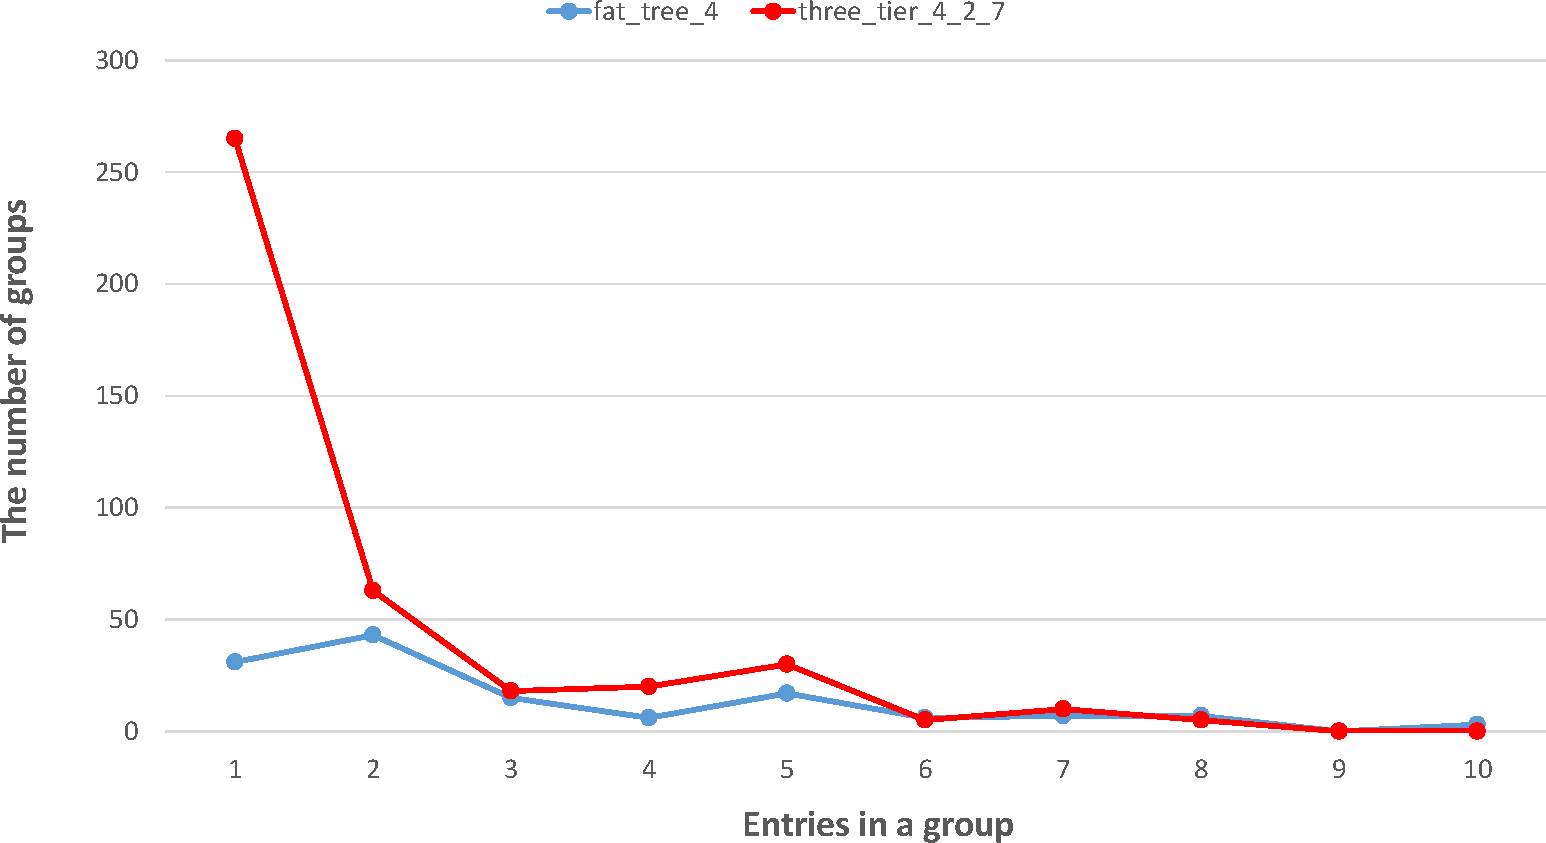
\includegraphics[width=1\textwidth]{figures/exp_topotype_distribute.pdf}
\caption{The comparison between fat\_tree\_4 and three\_tier\_4\_2\_7 -- the number of aggregated groups than contain various number of entries.}
\label{different_topo_distribute}
\end{figure}

\subsection{Influence of network scale}
To observe how effective our method is for various network scales, various sizes of fat-tree topology will be used. Fat-tree topologies are chosen for this experiment because the other two topology types have influence on the experimental result mostly by the way switches are connected. The parameter $n$ (i.e., the number of pods) ranges from 2 to 14. Since the network scale grows significantly with a larger number of pods, we consider at most 14 pods. There are also 20 entries on each switch. The results are shown in Table~\ref{table:different_scale}, and the trend chart of effective aggregation rates and actual aggregation rates are shown in Figure~\ref{different_scale_rate_trend}.

\begin{table}
\centering
\caption{Influence of various network scales}
\begin{tabular}{|l|p{2cm}|p{2.5cm}|p{1.9cm}|p{2.8cm}|}
\hline topology name & Effective aggregation rate & Actual aggregation rate & Execution time(sec) & Number of auxiliary entries \\
\hline
\hline fat\_tree\_2 & 2.70 & 2.84 & 1.26 & 35 \\
\hline fat\_tree\_4 & 2.96 & 3.27 & 8.27 & 142 \\
\hline fat\_tree\_6 & 2.85 & 3.27 & 19.16 & 327 \\
\hline fat\_tree\_8 & 2.81 & 3.29 & 33.03 & 589 \\
\hline fat\_tree\_10 & 2.91 & 3.37 & 51.81 & 921 \\
\hline fat\_tree\_12 & 2.89 & 3.36 & 74.78 & 1334 \\
\hline fat\_tree\_14 & 2.79 & 3.29 & 102.56 & 1800 \\
\hline
\end{tabular}
\label{table:different_scale}
\end{table}

In the trend chart of effective and actual aggregation rates in Figure~\ref{different_scale_rate_trend}, the aggregation rates are similar in various sizes of topology except fat\_tree\_2 which has lower aggregation rates due to fewer number of switches and links, and the scale does not have any clear effect on the aggregation rates. Theoretically, there should be positive and negative factors that will influence the aggregation rates. A positive factor, for example, is a larger number of links, which help to raise the chance of adopting an entry into a group if the ratio between the number of forwarding ports and entries are balanced. Some examples of negative factors are more entries to be fit into aggregated groups and more hosts that will stop an aggregated group from extension. The result shows that these factors break even, and the effectiveness of our method will not drop with the increasing topology size.

\begin{figure}[H]
\centering
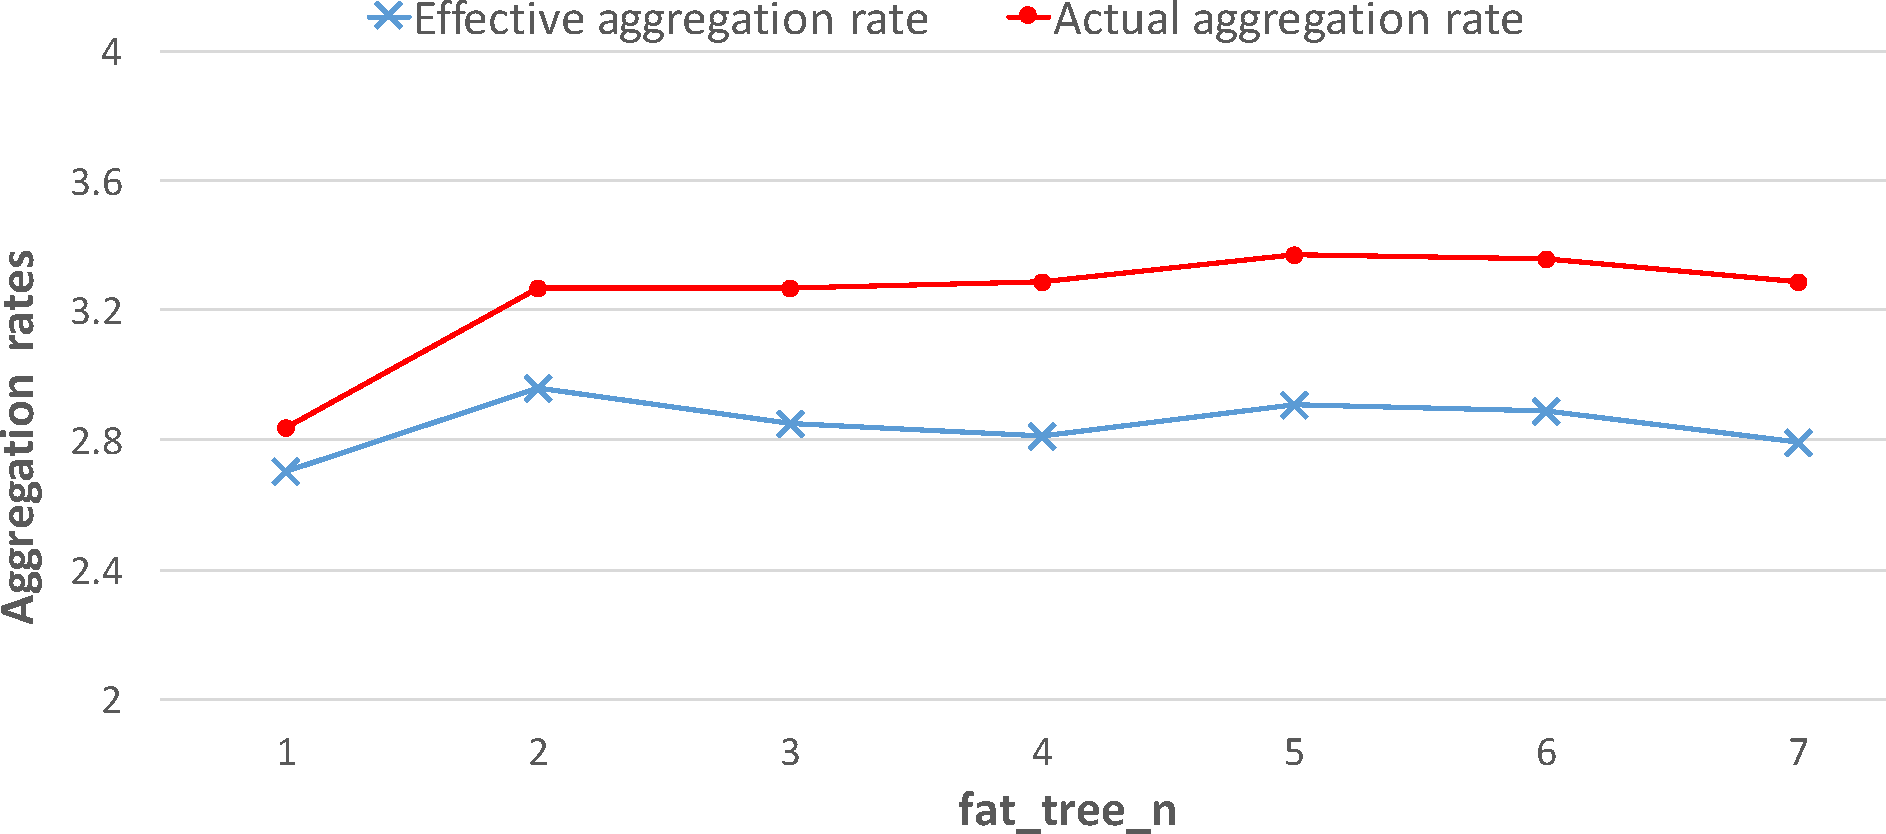
\includegraphics[width=1\textwidth]{figures/exp_scale_rate_trend.pdf}
\caption{The trend chart of aggregation rates under various scales of network.}
\label{different_scale_rate_trend}
\end{figure}

The relation between the topology size and the execution time is presented in Figure~\ref{different_scale_time_trend}, and the relation between the topology size and the number of auxiliary entries is presented in Figure~\ref{different_scale_aux_trend}. As we can see, both trends look pretty similar, and they are proportional to $n^2$. It is quite as expected since the growth rate of switch is also proportional to $n^2$.

\begin{figure}[H]
\centering 
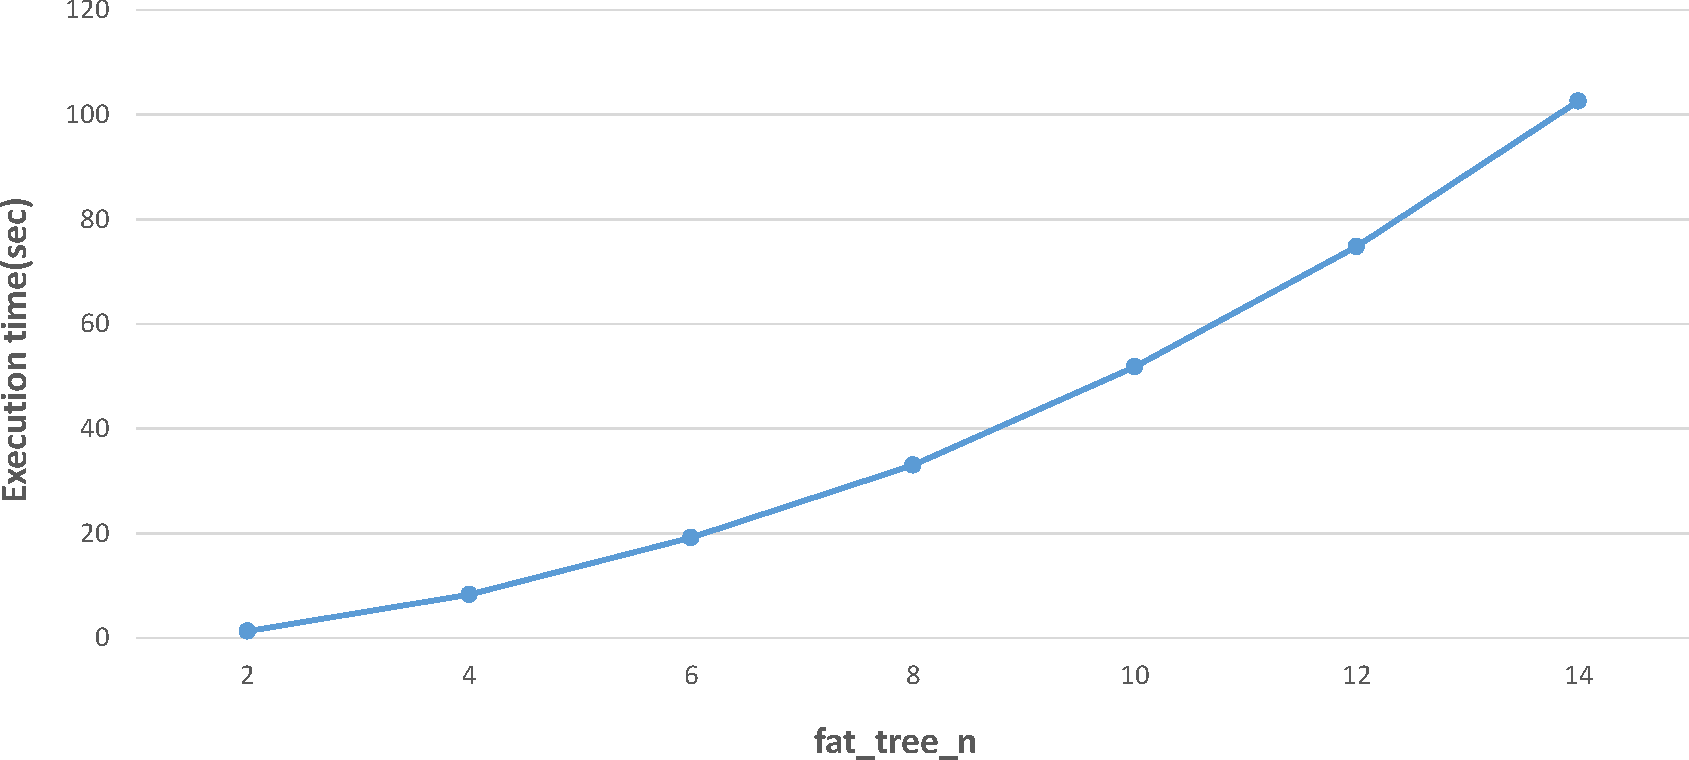
\includegraphics[width=1\textwidth]{figures/exp_scale_time_trend.pdf}
\caption{The trend chart of execution time under various scales of network.}
\label{different_scale_time_trend}
\end{figure}

\begin{figure}[H]
\centering 
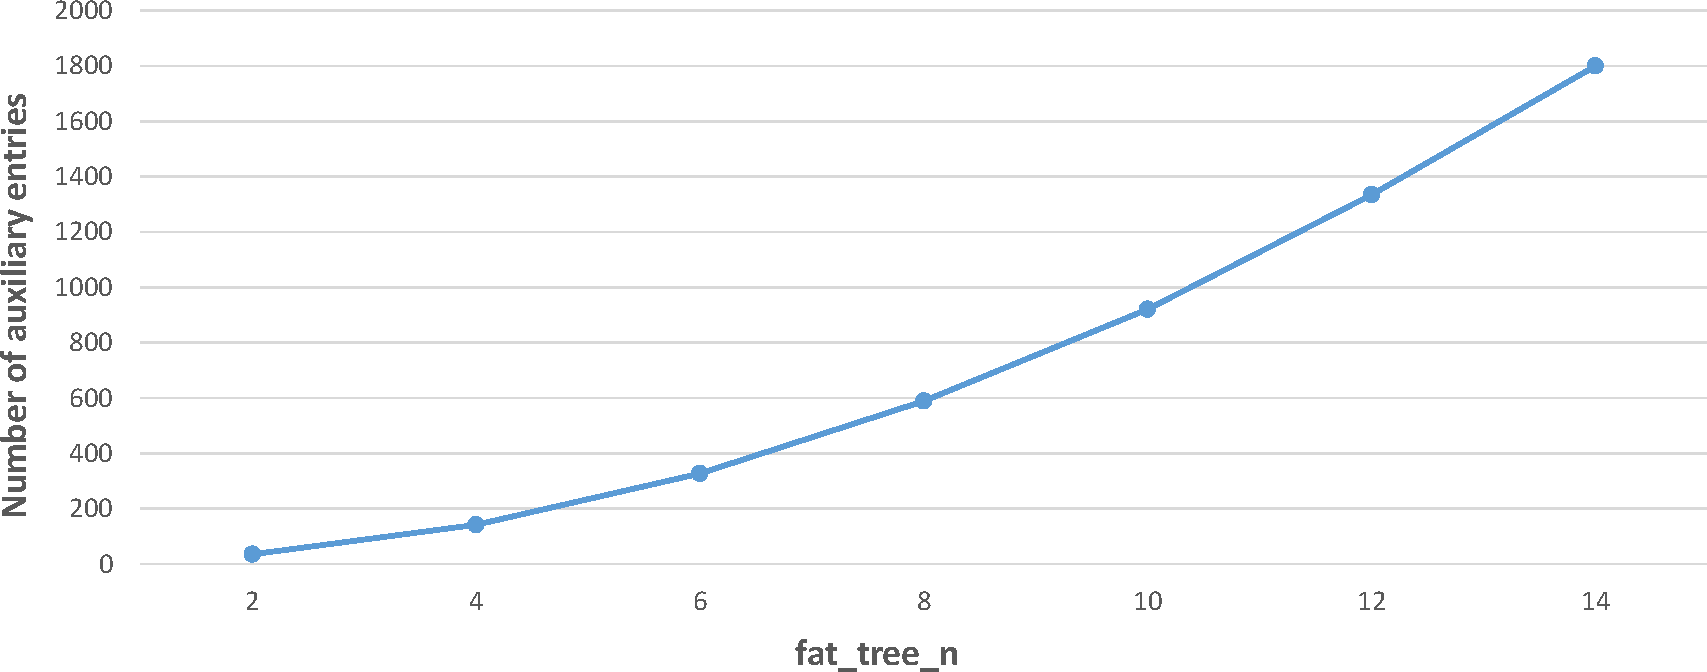
\includegraphics[width=1\textwidth]{figures/exp_scale_aux_trend.pdf}
\caption{The trend chart of number of auxiliary entries under various scales of network.}
\label{different_scale_aux_trend}
\end{figure}

\subsection{Influence of flow entry number on each switch}
In this experiment, we will use only one topology -- fat\_tree\_4, and change the number of entries on each switch to see the influence it may bring. The number of entries on each switch increases from 10 to 200, and the intervals of entry number on each switch between every run increase as the number of entries on each switch grows, and the trend chart of effective aggregation rate with various number of entries on each switch is shown in Figure~\ref{exp_entrynum_trend}. The execution time and the number of auxiliary entries grow roughly linearly along with the number of entries on a switch.

\begin{table}
\centering
\caption{Aggregation rates, execution time and number of auxiliary entries for various number of entries on a switch.}
\begin{tabular}{|p{1.8cm}|p{2.6cm}|p{2.6cm}|p{1.9cm}|p{2.8cm}|}
\hline Number of entries per switch & Effective aggregation rate & Actual aggregation rate & Execution time (sec) & Number of auxiliary entries \\
\hline
\hline 10 & 2.38 & 3.15 & 3.98 & 72 \\
\hline 20 & 2.96 & 3.27 & 8.27 & 142 \\
\hline 30 & 3.01 & 3.64 & 15.03 & 214 \\
\hline 40 & 3.04 & 4.03 & 19.24 & 280 \\
\hline 50 & 3.18 & 4.22 & 26.19 & 346 \\
\hline 65 & 3.35 & 4.45 & 34.31 & 461 \\
\hline 80 & 3.41 & 4.51 & 41.47 & 560 \\
\hline 100 & 3.43 & 4.47 & 55.58 & 672 \\
\hline 120 & 3.48 & 4.45 & 64.96 & 812 \\
\hline 160 & 3.60 & 4.69 & 89.21 & 1070 \\
\hline 200 & 3.60 & 4.62 & 119.47 & 1359 \\
\hline 
\end{tabular}
\label{table:different_entry_per_switch}
\end{table}

\begin{figure}
\centering
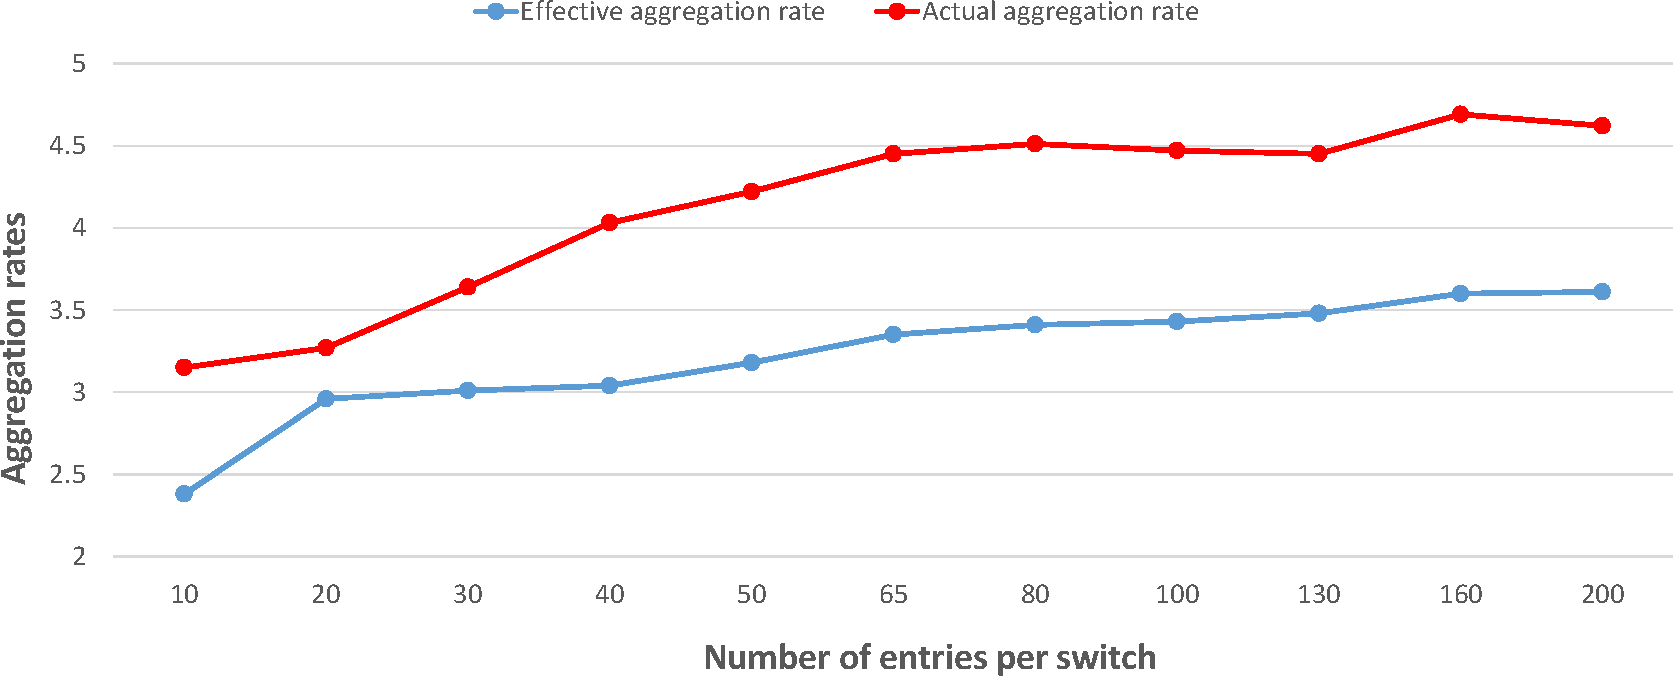
\includegraphics[width=1\textwidth]{figures/exp_entrynum_trend.pdf}
\caption{The trend chart of effective aggregation rate and actual aggregation rate with various number of entries per switch.}
\label{exp_entrynum_trend}
\end{figure}

From the trend chart in Figure~\ref{exp_entrynum_trend}, we can clearly see that the aggregation rates grow as the number of entries in the switch increases from 5 to 50 entries per switch. However, the growth rate decreases slowly after 50 entries per switch as the number of entries gets larger. A reasonable explanation for this phenomenon is the limited number of fields in a detection packet. Two fields can be selected at each L2/L3/L4 layer at most. For example, after entries with the match fields ``source IP'' and ``destination IP'', which are both at IP layer, are chosen into an aggregated group, it is impossible to add another entry whose match field is also at IP layer. Hence, a detection packet is able to accommodate no more than 6 fields and values. Since effective aggregation rate means the average number of entries in the aggregated groups, from this perspective, we may infer that the effective aggregation rate should converge at 6 if the number of entries on each switch gets really large. We refer to a packet with 6 fields and values set as a saturated packet.

\subsection{Examination and discussion}
\label{examination_and_discussion}

Before the experiment, we expect that the higher degree it is, the higher chance that we are able to extend an aggregated group more, which will result in higher aggregation rates. However, according to the result in Table~\ref{table:different_topo_type}, it seems that it is not always true, since the two-tier topologies have the highest average degree overall but has a moderate result. The fat-tree topology has the best result, while the three-tier topologies tend to have the worse result. After tracking down the entries inside the two-tier topologies, we discover that although the number of degrees is high, the ratio between the number of forwarding ports and the number of entries is imbalanced. The ports for forwarding to the neighbors are uniformly distributed among the entries, and they indicate the forwarding paths to choose while finding an aggregated group. There are not as many paths as we expect for an aggregated group to choose during entry selection, and thus the aggregation rates of two-tier topologies are lower than those of the fat-tree topology. 

To justify the inference that the effective aggregation rate may converge at 6 if the number of entries on each switch gets large, we also conducted another run of experiment with 1000 entries on each switch. Different from the inference, it results in an effective aggregation rate of 4.46 and an actual aggregation rate of 5.87. After further inspecting the content in aggregated groups, we discover that due to how the \texttt{tcp\_port} field is generated, there are many entries with TCP source or destination 80. When these entries are met during the group finding process, it is likely for two aggregated groups to end up in the same location once the two groups pass through the same switch during the finding process. As a detection packet gets closer to saturation, it will also make it harder for the corresponding aggregated group to find another entry that satisfies the aggregation conditions. Therefore, we did not have the best effective aggregation rate even with a large number of entries per switch. 

From the above experiments and analysis, we have the following conclusions. First, although the network scales are the same, the way how the switches are connected to each other leads to significant differences. Second, the network scale does not have clear influence on the efficiency of the detection method. Last but not the least, the more entries there are in the switches, the higher aggregation rates we are able to get; but as the average effective aggregation rate get closer and closer to 6, the aggregation rates grow slower and slower. We can conclude that the detection method is effective. Moreover, in our experimental environments, the structures are at most three tiers, which means in real-case network structures with more tiers, the method can be even more effective. 